\documentclass{beamer}

\usepackage[utf8]{inputenc}
\usepackage{forest}
\usepackage{tikz}
\usepackage{amsmath}
\usetikzlibrary{arrows,automata,positioning,backgrounds}

\usetheme{default}
\beamertemplatenavigationsymbolsempty

\title{Ungleichungen von Kraft \& McMillan}
\subtitle{Proseminar Informationstheorie}
\author{Phil Pützstück}
\date{\today}

\newcommand{\up}[2]{\mathrel{\overset{\makebox[0pt]{\mbox{\normalfont\tiny #2}}}{#1}}}

\forestset{%
  only/.code args={<#1>}{%
    \alt<#1>{}{\pgfkeysalso{before typesetting nodes={remove}}}
  },
}

\begin{document}
\maketitle

\section{Bäume}
%\begin{frame}
%    \frametitle{Motivation}
%    \begin{itemize}
%        \setlength\itemsep{2em}
%        \item Gesehen, dass eindeutig bzw. sofort dekodierbare Codes sehr nützlich sind.
%        \item Wann bzw. unter welchen Bedingungen existieren diese?
%        \item Insbesondere: Wortlängen und Größe des Code-Alphabets
%        \item Vorgestellte Ungleichungen geben untere Schranken für diese
%    \end{itemize}
%\end{frame}
%
%\begin{frame}
%    \frametitle{Überblick}
%    \begin{itemize}
%        \setlength\itemsep{2em}
%        \item Zusammenhang Codes und Bäume
%        \item Ungleichung von Kraft
%        \item Ungleichung von McMillan
%        \item Intepretationen / Ausblick
%    \end{itemize}
%\end{frame}
%
%\begin{frame}[t]
%    \frametitle{Code als Baum: $\mathcal{T}_r^h$}
%    Höhe $h \in \mathbb{N}$, Verzweigungsgrad $r \in \mathbb{N}$.
%    \begin{center}
%        \only<1-2>{
%        \Large
%        \begin{forest}
%            [$v_\varepsilon$
%                [$v_0$
%                    [$v_{00}$],
%                    [$v_{01}$],
%                    [$v_{02}$]
%                ],
%                [$v_1$
%                    [$v_{10}$],
%                    [$v_{11}$],
%                    [$v_{12}$]
%                ],
%                [$v_2$
%                    [$v_{20}$],
%                    [$v_{21}$],
%                    [$v_{22}$]
%                ]
%            ],
%        \end{forest}\\
%        }
%        \only<3->{
%        \Large
%        \begin{forest}
%            [\LARGE $v_{\color{red}\varepsilon}$
%                [$v_0$
%                    [$v_{00}$],
%                    [$v_{01}$],
%                    [$v_{02}$]
%                ],
%                [\LARGE $v_{\color{red}1}$, edge label={node [midway, sloped, above] {\color{blue}$\geq$}}
%                    [\LARGE$v_{{\color{red}1}0}$, edge label={node [midway, sloped, above] {\color{blue}$\geq$}}],
%                    [\LARGE$v_{{\color{red}1}1}$, edge label={node [midway, sloped, above] {\normalsize\color{blue}$\leq$}}],
%                    [\LARGE$v_{{\color{red}1}2}$, edge label={node [midway, sloped, above] {\color{blue}$\leq$}}]
%                ],
%                [$v_2$
%                    [$v_{20}$],
%                    [$v_{21}$],
%                    [$v_{22}$]
%                ]
%            ],
%        \end{forest}\\
%        }
%    \end{center}
%    \pause
%    \begin{itemize}
%        \setlength\itemsep{2em}
%        \item Für $v_w \in V(\mathcal{T}_r^h)$ gilt $height(v_w) = |w|$.
%        \pause
%        \item Für $v_w, v_{w'} \in V(\mathcal{T}_r^h)$ gilt
%            $v_w\ {\color{blue}\leq}\ v_{w'} \,\Longleftrightarrow\, w\ {\color{red}\sqsubseteq}\ w'$.
%    \end{itemize}
%\end{frame}
%
%\section{Ungleichung von Kraft}
%\begin{frame}
%    \frametitle{Ungleichung von Kraft}
%    Seien $q,r \in \mathbb{N}, \ell \in \mathbb{N}^q$. Dann existiert ein $r$-ärer sofort dekodierbarer Code $\mathcal{C}$
%    mit Wortlängen $\ell$ genau dann, wenn
%    $$
%        \sum_{k=1}^{q} \frac{1}{r^{\ell_k}} \leq 1
%    $$\\[20pt]
%    \pause
%
%    Annahmen:
%
%    \begin{itemize}
%        \setlength\itemsep{1em}
%        \item Anzahl Code-Wörter $q > 1$
%        \pause
%        \item Wortlängen $0 < \ell_1 \leq \ell_2 \leq \cdots \leq \ell_q$
%            aufsteigend sortiert
%        \pause
%        \item Code-Alphabet von $\mathcal{C}$ ist $[0,r-1]$
%    \end{itemize}
%\end{frame}
%
%\begin{frame}[t]
%    \frametitle{Ungleichung von Kraft: Beweisidee ''$\,\Longrightarrow\,$''}
%    Richtung ''$\sum_{k=1}^{q} \frac{1}{r^{\ell_k}} \leq 1 \,\Longrightarrow\,$ $\mathcal{C}$ existiert''.\\[5pt]
%    \pause
%    Bekannt: $\mathcal{C}$ sofort dekodierbar $\,\Longleftrightarrow\,$ $\mathcal{C}$ Präfixcode.\\[5pt]
%    \pause
%    Beispiel:
%    $
%    q=3,
%    {\only<4>{\color{red}}r=2},
%    \ell=(
%    {\only<5>{\color{blue}}1},
%    {\only<9>{\color{blue}}2},
%    {\only<4,13>{\color{blue}}3})
%    $.
%    \only<15>{\\$w_1=0$,\ \ $w_2=11$,\ $w_3=101$}
%    \only<4-14>{
%        Betrachte
%        \only<4-7>{$\mathcal{T}_{\only<4>{\color{red}}2}^{\only<4>{\color{blue}}3}$}
%        \only<8-11>{{\only<8>{\color{red}}$\mathcal{T}_2^3 \setminus v_0$}}
%        \only<12-14>{{\only<12>{\color{red}}$(\mathcal{T}_2^3 \setminus v_0) \setminus v_{11}$}}
%        \\
%        \only<6-14>{
%            {\only<6>{\color{blue}}$w_1 = {\only<7>{\color{red}}0}$},
%            \only<10-14>{
%                {\only<10>{\color{blue}}$w_2 = {\only<11>{\color{red}}11}$},
%                \only<14>{{\color{blue}$w_3 = 101$}}
%            }
%        }
%    }
%    \strut\\[20pt]
%    \onslide{
%        \only<4>{
%            \begin{center}
%                \begin{forest}
%                    [$v_\varepsilon$
%                        [$v_0$
%                            [$v_{00}$
%                                [$v_{000}$],
%                                [$v_{001}$]
%                            ],
%                            [$v_{01}$
%                                [$v_{010}$],
%                                [$v_{011}$]
%                            ]
%                        ],
%                        [$v_1$
%                            [$v_{10}$
%                                [$v_{100}$],
%                                [$v_{101}$]
%                            ],
%                            [$v_{11}$
%                                [$v_{110}$],
%                                [$v_{111}$]
%                            ]
%                        ]
%                    ]
%                \end{forest}
%            \end{center}
%        }
%        \only<5>{
%            \begin{center}
%                \begin{forest}
%                    [$v_\varepsilon$
%                        [$v_0$,blue,draw
%                            [$v_{00}$
%                                [$v_{000}$],
%                                [$v_{001}$]
%                            ],
%                            [$v_{01}$
%                                [$v_{010}$],
%                                [$v_{011}$]
%                            ]
%                        ],
%                        [$v_1$,blue,draw
%                            [$v_{10}$
%                                [$v_{100}$],
%                                [$v_{101}$]
%                            ],
%                            [$v_{11}$
%                                [$v_{110}$],
%                                [$v_{111}$]
%                            ]
%                        ]
%                    ]
%                \end{forest}
%            \end{center}
%        }
%        \only<6>{
%            \begin{center}
%                \begin{forest}
%                    [$v_\varepsilon$
%                        [$v_0$,draw,blue
%                            [$v_{00}$
%                                [$v_{000}$],
%                                [$v_{001}$]
%                            ],
%                            [$v_{01}$
%                                [$v_{010}$],
%                                [$v_{011}$]
%                            ]
%                        ],
%                        [$v_1$
%                            [$v_{10}$
%                                [$v_{100}$],
%                                [$v_{101}$]
%                            ],
%                            [$v_{11}$
%                                [$v_{110}$],
%                                [$v_{111}$]
%                            ]
%                        ]
%                    ]
%                \end{forest}
%            \end{center}
%        }
%        \only<7>{
%            \begin{center}
%                \begin{forest}
%                    [$v_\varepsilon$
%                        [$v_{\color{red}0}$
%                            [$v_{{\color{red}0}0}$
%                                [$v_{{\color{red}0}00}$],
%                                [$v_{{\color{red}0}01}$]
%                            ],
%                            [$v_{{\color{red}0}1}$
%                                [$v_{{\color{red}0}10}$],
%                                [$v_{{\color{red}0}11}$]
%                            ]
%                        ],
%                        [$v_1$
%                            [$v_{10}$
%                                [$v_{100}$],
%                                [$v_{101}$]
%                            ],
%                            [$v_{11}$
%                                [$v_{110}$],
%                                [$v_{111}$]
%                            ]
%                        ]
%                    ]
%                \end{forest}
%            \end{center}
%        }
%        \only<8>{
%            \begin{center}
%                \begin{forest}
%                    [$v_\varepsilon$
%                        [$v_0$,red,edge={dashed},
%                            [$v_{00}$,red
%                                [$v_{000}$,red],
%                                [$v_{001}$,red]
%                            ],
%                            [$v_{01}$,red
%                                [$v_{010}$,red],
%                                [$v_{011}$,red]
%                            ]
%                        ],
%                        [$v_1$
%                            [$v_{10}$,
%                                [$v_{100}$],
%                                [$v_{101}$]
%                            ],
%                            [$v_{11}$,
%                                [$v_{110}$],
%                                [$v_{111}$]
%                            ]
%                        ]
%                    ]
%                \end{forest}
%            \end{center}
%        }
%        \only<9>{
%            \begin{center}
%                \begin{forest}
%                    [$v_\varepsilon$
%                        [$v_0$,red,edge={dashed},
%                            [$v_{00}$,red,draw,dashed
%                                [$v_{000}$,red],
%                                [$v_{001}$,red]
%                            ],
%                            [$v_{01}$,red,draw,dashed
%                                [$v_{010}$,red],
%                                [$v_{011}$,red]
%                            ]
%                        ],
%                        [$v_1$
%                            [$v_{10}$,draw,blue
%                                [$v_{100}$],
%                                [$v_{101}$]
%                            ],
%                            [$v_{11}$,draw,blue
%                                [$v_{110}$],
%                                [$v_{111}$]
%                            ]
%                        ]
%                    ]
%                \end{forest}
%            \end{center}
%        }
%        \only<10>{
%            \begin{center}
%                \begin{forest}
%                    [$v_\varepsilon$
%                        [$v_0$,red,edge={dashed},
%                            [$v_{00}$,red
%                                [$v_{000}$,red],
%                                [$v_{001}$,red]
%                            ],
%                            [$v_{01}$,red
%                                [$v_{010}$,red],
%                                [$v_{011}$,red]
%                            ]
%                        ],
%                        [$v_1$
%                            [$v_{10}$,
%                                [$v_{100}$],
%                                [$v_{101}$]
%                            ],
%                            [$v_{11}$,draw,blue
%                                [$v_{110}$],
%                                [$v_{111}$]
%                            ]
%                        ]
%                    ]
%                \end{forest}
%            \end{center}
%        }
%        \only<11>{
%            \begin{center}
%                \begin{forest}
%                    [$v_\varepsilon$
%                        [$v_0$,red,edge={dashed}
%                            [$v_{00}$,red
%                                [$v_{000}$,red],
%                                [$v_{001}$,red]
%                            ],
%                            [$v_{01}$,red
%                                [$v_{010}$,red],
%                                [$v_{011}$,red]
%                            ]
%                        ],
%                        [$v_1$
%                            [$v_{10}$
%                                [$v_{100}$],
%                                [$v_{101}$]
%                            ],
%                            [$v_{\color{red}11}$
%                                [$v_{{\color{red}11}0}$],
%                                [$v_{{\color{red}11}1}$]
%                            ]
%                        ]
%                    ]
%                \end{forest}
%            \end{center}
%        }
%        \only<12>{
%            \begin{center}
%                \begin{forest}
%                    [$v_\varepsilon$
%                        [$v_0$,red,edge={dashed}
%                            [$v_{00}$,red
%                                [$v_{000}$,red],
%                                [$v_{001}$,red]
%                            ],
%                            [$v_{01}$,red
%                                [$v_{010}$,red],
%                                [$v_{011}$,red]
%                            ]
%                        ],
%                        [$v_1$
%                            [$v_{10}$
%                                [$v_{100}$],
%                                [$v_{101}$]
%                            ],
%                            [$v_{11}$,red,edge={dashed}
%                                [$v_{110}$,red],
%                                [$v_{111}$,red]
%                            ]
%                        ]
%                    ]
%                \end{forest}
%            \end{center}
%        }
%        \only<13>{
%            \begin{center}
%                \begin{forest}
%                    [$v_\varepsilon$
%                        [$v_0$,red,edge={dashed}
%                            [$v_{00}$,red
%                                [$v_{000}$,red,draw,dashed],
%                                [$v_{001}$,red,draw,dashed]
%                            ],
%                            [$v_{01}$,red
%                                [$v_{010}$,red,draw,dashed],
%                                [$v_{011}$,red,draw,dashed]
%                            ]
%                        ],
%                        [$v_1$
%                            [$v_{10}$
%                                [$v_{100}$,draw,blue],
%                                [$v_{101}$,draw,blue]
%                            ],
%                            [$v_{11}$,red,edge={dashed}
%                                [$v_{110}$,red,draw,dashed],
%                                [$v_{111}$,red,draw,dashed]
%                            ]
%                        ]
%                    ]
%                \end{forest}
%            \end{center}
%        }
%        \only<14>{
%            \begin{center}
%                \begin{forest}
%                    [$v_\varepsilon$
%                        [$v_0$,red,edge={dashed}
%                            [$v_{00}$,red
%                                [$v_{000}$,red],
%                                [$v_{001}$,red]
%                            ],
%                            [$v_{01}$,red
%                                [$v_{010}$,red],
%                                [$v_{011}$,red]
%                            ]
%                        ],
%                        [$v_1$
%                            [$v_{10}$
%                                [$v_{100}$],
%                                [$v_{101}$,draw,blue]
%                            ],
%                            [$v_{11}$,red,edge={dashed}
%                                [$v_{110}$,red],
%                                [$v_{111}$,red]
%                            ]
%                        ]
%                    ]
%                \end{forest}
%            \end{center}
%        }
%        \only<15->{
%            \begin{itemize}
%                \setlength\itemsep{1.5em}
%                \item $q = 3$ Wörter über Alphabet $[0,r-1] = [0,1] = \{0,1\}$.
%                \item Wortlängen $|w_1| = \ell_1, |w_2| = \ell_2, |w_3| = \ell_3$ eingehalten.
%                \item Präfixcode $\mathcal{C} = \{w_1,w_2,w_3\} = \{0,11,101\}$ konstruiert.
%            \end{itemize}
%        }
%    }
%\end{frame}
%
%\begin{frame}
%    \frametitle{Ungleichung von Kraft ''$\,\Longrightarrow\,$'': Induktionsanfang}
%    \begin{columns}
%    \begin{column}{0.7\textwidth}
%        \visible<1->{
%            \begin{itemize}
%                \setlength\itemsep{1em}
%                \item zz: Auswahl von $w_i$ aus Baum möglich.
%                \item Via endlicher Induktion über $i$.
%                \item $h := \ell_q$ (max. Wortlänge)
%            \end{itemize}\strut\\[20pt]\pause
%
%            $i=1$:\\
%
%            \begin{itemize}
%                \setlength\itemsep{1em}
%                \item Wähle
%                    ${\only<2>{\color{red}}v_w} \in V(\mathcal{T}_r^h), height({\only<2>{\color{red}}v_w}) = \ell_1$
%                \pause
%                \item Setze $w_1 := w$, dann $|w_1| = \ell_1$
%                \pause
%                \item Entferne Nachfolger; $\mathcal{T} := \mathcal{T}_r^h \setminus v_w$
%            \end{itemize}
%        }
%    \end{column}
%
%    \begin{column}{0.3\textwidth}
%        \onslide
%        \visible<2->{
%            \quad$\mathcal{T}_r^h$:\\
%            \begin{center}
%                \begin{forest}
%                    [$v_\varepsilon$
%                        [$v_0$,
%                            [\dots]
%                        ],
%                        [$v_1$
%                            [\dots
%                                [$v_w$,only=<2-3>,color=red,
%                                    [$v_{w0}$
%                                        [\dots]
%                                    ],
%                                    [$v_{w1}$
%                                        [\dots]
%                                    ],
%                                    [\dots]
%                                ],
%                                [$v_w$,only=<4>,color=red,edge={dashed,red}
%                                    [$v_{w0}$,red
%                                        [\dots,red]
%                                    ],
%                                    [$v_{w1}$,red
%                                        [\dots,red]
%                                    ],
%                                    [\dots,red]
%                                ],
%                            ],
%                            [\dots]
%                        ],
%                        [\dots]
%                    ]
%                \end{forest}
%            \end{center}
%        }
%    \end{column}
%    \end{columns}
%\end{frame}
%
%\begin{frame}[t]
%    \frametitle{Ungleichung von Kraft ''$\,\Longrightarrow\,$'': Induktionsanfang}
%    \begin{columns}
%    \begin{column}{0.5\textwidth}
%        \visible<1->{
%            \begin{itemize}
%                \setlength\itemsep{1em}
%                \item Teilbaum der Höhe $\ell_1$ entfernt
%                \pause
%                \item $\mathcal{T}_1$ noch $r^h - r^{h-\ell_1}$ Blätter
%            \end{itemize}\strut\\[10pt]\pause
%        }
%        Weiter gilt:
%        \begin{overprint}
%            \onslide<3>
%            $$
%                r^h - r^{h - \ell_1} = r^h\bigg(1 - \sum_{k=1}^{1} \frac{1}{r^{\ell_k}}\bigg)
%            $$
%            \onslide<4>
%            $$
%                r^h - r^{h - \ell_1} = r^h\bigg(1 - \sum_{k=1}^{1} \frac{1}{r^{\ell_k}}\bigg)
%            $$
%            $$
%                {>}\ r^h\bigg(1 - \sum_{k=1}^{q} \frac{1}{r^{\ell_k}}\,\bigg )\visible<5>{> 0}
%            $$
%            \onslide<5>
%            $$
%                r^h - r^{h - \ell_1} = r^h\bigg(1 - \sum_{k=1}^{1} \frac{1}{r^{\ell_k}}\bigg)
%            $$
%            $$
%                {\color{red} >}\ r^h\bigg(1 - \underbrace{\sum_{k=1}^{q} \frac{1}{r^{\ell_k}}}_{\leq\ 1}\bigg)
%                > {\color{red}0}
%            $$
%        \end{overprint}
%    \end{column}
%
%        \begin{column}{0.55\textwidth}
%        \onslide
%            \begin{center}
%                \begin{tikzpicture}
%                    \only<1>{\node[color=red] at (0.5,-3) {$v_{w_1}$};}
%                    \only<2->{\node at (0.5,-3) {$v_{w_1}$};}
%                    \node at (0,-1.5) {$\mathcal{T}_1$};
%
%                    \draw (0,0) node[above]{$v_\varepsilon$}
%                        -- (-2.5,-4)
%                        -- (-.5,-4)
%                        -- (0.5,-2.4)
%                        -- (1.5,-4)
%                        -- (2.5,-4)
%                        -- cycle;
%
%                    \draw[|-|] (3,-2.4) -- node[left] {$\ell_1$} (3, 0);
%                    \draw[|-|] (3,-2.4) -- node[left] {\scriptsize{$h-\ell_1$}} (3, -4);
%                    \draw[dotted, line width = .6pt] (3,-2.4) -- (0.5,-2.4);
%                    \draw[dotted, line width = .6pt] (3,0) -- (0,0);
%                    \draw[dotted, line width = .6pt] (2.5,-4) -- (3,-4);
%                    \visible<2->{
%                        \draw[|-|] (-.5,-4.5) -- node[below] {$r^{h-\ell_1}$} (1.5,-4.5);
%                        \draw[|-|] (-2.5,-5.4) -- node[below] {$r^h$} (2.5,-5.4);
%                    }
%                \end{tikzpicture}
%            \end{center}
%    \end{column}
%    \end{columns}
%\end{frame}

%\begin{frame}[t]
%    \frametitle{Ungleichung von Kraft: ''$\,\Longrightarrow\,$'': Induktionsschritt}
%
%    \begin{columns}
%    \begin{column}{0.7\textwidth}
%        Vorraussetzungen für $i \in [1,q-1]$:
%        \begin{itemize}
%            \setlength\itemsep{.8em}
%            \item $\forall j \in [1,i]: |w_j| = \ell_j$
%            \item $\{w_j \mid j \in [1,i]\}$ Präfix-Code
%            \item $|leaves(\mathcal{T}_j)| > 0$
%        \end{itemize}\strut\\[10pt]
%        \pause
%        Dann:
%        \begin{itemize}
%            \setlength\itemsep{.8em}
%            \item Es gibt Blatt $v_x \in V(\mathcal{T}_i)$.
%            \item $\mathcal{T}_i$ als Baum zusammenhängend
%            \pause
%            \item $\exists v_w \in V(\mathcal{T}_i): height(v_w) = \ell_{i+1} \leq h$
%            \pause
%            \item Setze $w_{i+1} := w$. Dann $|w_{i+1}| = \ell_{i+1}$
%        \end{itemize}
%    \end{column}
%    \begin{column}{0.3\textwidth}\onslide
%        \only<2->{
%        \begin{center}
%            \begin{tikzpicture}
%                \node at (0,0) {$v_\varepsilon$};
%                \node at (0,-4) {$v_x$};
%                \visible<3->{\node[blue] at (0,-2) {$v_w$};}
%
%                \draw[dotted,line width = 1pt] (0,-0.5) -- (0,-1.5);
%                \visible<2>{\draw[dotted,line width = 1pt] (0,-0.5) -- (0,-2.5);}
%                \draw[dotted,line width = 1pt] (0,-2.5) -- (0,-3.5);
%
%                \visible<3->{\draw[|-|] (.5, 0) -- node[right] {$\ell_{i+1}$}(.5, -2);}
%                \draw[|-|] (1.5, 0) -- node[right] {$h$}(1.5, -4);
%            \end{tikzpicture}
%        \end{center}
%        }
%    \end{column}
%    \end{columns}
%\end{frame}
%
%\begin{frame}[t]
%    \frametitle{Ungleichung von Kraft: ''$\,\Longrightarrow\,$'': Induktionsschritt}
%    Für $j \in [1,i]$:
%    \begin{itemize}
%        \setlength\itemsep{1em}
%        \item Knoten ''unter'' $v_{w_j}$ bereits entfernt
%        \pause
%        \item Damit $v_{w_j} \not\leq v_{w_{i+1}}$, also auch $w_j \not\sqsubseteq w_{i+1}$
%        \pause
%        \item Ausserdem $w_{i+1} \not\sqsubseteq w_{j}$ durch $|w_j| = \ell_j \leq \ell_{i+1} = |w_{i+1}|$
%    \end{itemize}
%
%    \begin{center}\onslide
%        \begin{tikzpicture}[scale=.9]
%            \node[color=red] at (2,-4) {$v_{w_1}$};
%            \node[color=red] at (-4.5,-5) {$v_{w_j}$};
%            \node[color=red] at (-2.5,-5.2) {$v_{w_k}$};
%            \node[color=blue] at (-0.2,-5) {$v_{w_{i+1}}$};
%            \node at (-1,-5.8) {$v_x$};
%            \node at (0,-1.5) {$\mathcal{T}_i$};
%
%            \draw (0,0)
%                -- (-4.5,-4.5)
%                -- (-3.5,-5.5)
%                -- (-3.25,-5.5)
%                -- (-2.5,-4.75)
%                -- (-1.75,-5.5)
%                -- (0,-5.5)
%                -- (2,-3.5)
%                -- (4,-5.5)
%                -- (5.5,-5.5)
%                -- cycle;
%
%            \draw[dashed] (0,0)
%                -- (0,-0.15)
%                -- (-1,-1.15)
%                -- (0,-2)
%                -- (-1.5,-3.5)
%                -- (-1,-4)
%                -- (-1.25,-4.25)
%                -- (-0.5,-5)
%                -- (-1,-5.5);
%        \end{tikzpicture}
%    \end{center}
%\end{frame}
%
%\begin{frame}[t]
%    \frametitle{Ungleichung von Kraft: ''$\,\Longrightarrow\,$'': Induktionsschritt}
%    \begin{itemize}
%        \setlength\itemsep{1em}
%        \item Damit $\{w_j \mid j \in [1,{\color{blue}i+1}]\}$ wieder Präfix-Code.
%        \pause
%        \item Falls $i+1 = q$: Setze $\mathcal{C} := \{w_j \mid j \in [1,i+1]\}$.
%        \pause
%        \item Falls $i+1 < q$: Entferne Nachfolger: $\mathcal{T}_{i+1} := \mathcal{T}_i \setminus v_{w_{i+1}}$
%        \pause
%        \item Dann $|leaves(\mathcal{T}_{i+1})| > 0$, denn:
%    \end{itemize}
%    \visible<4->{
%        $$
%            r^h - \sum_{k=1}^{i+1} r^{h-\ell_k}
%            \visible<5->{
%                \quad{\color{red}>}\quad r^h - \sum_{k=1}^{q} r^{h-\ell_k}
%            }
%        $$
%        \visible<6->{
%            $$
%                =\ r^h \bigg(1 - \underbrace{\sum_{k=1}^{q} \frac{1}{r^{\ell_k}}}_{\leq\ 1}\bigg)
%                \ \geq\ {\color{red}0}
%            $$
%        }
%    }\strut
%    \visible<7->{
%        Vorraussetzungen für I.S. erfüllt, also Induktion vollendet.\\
%        \ \ Sofort dekodierbares $\mathcal{C}$ für $q,r,l$ konstruierbar.\hfill$\square$
%    }
%\end{frame}

\begin{frame}[t]
    \frametitle{Ungleichung von Kraft: ''$\,\Longleftarrow\,$''}
    Zeige: $\mathcal{C}$ sofort dekodierbar $\,\Longrightarrow\,$ 
    Ungleichung gilt für Parameter
    \visible<2->{
        $$
            {\color{red}L_i} := \{v \in V(\mathcal{T}_r^h) \mid v_{w_i} \leq v \land height(v) = h\}
        $$
        \begin{center}\onslide
            \begin{tikzpicture}
                \node at (0,-1) {$\mathcal{T}_r^h$};
                \node at (.5, -2.3) {$v_{w_i}$};
                \node[color=red] at (.5, -4.3) {$L_i$};

                \draw (0,0)
                    -- (-4,-4)
                    -- (4,-4)
                    -- cycle;

                \draw[dashed] (-1,-4) -- (.5, -2.5) -- (2,-4);

                \draw[line width = 2pt, color=red] (-1,-4) -- (2,-4);
            \end{tikzpicture}
        \end{center}
        \visible<3>{
            \begin{itemize}
                \item Für $i,j \in [1,q]: i \neq j \,\Longrightarrow\, L_i \cap L_j = \varnothing$
            \end{itemize}
        }
    }
\end{frame}

\begin{frame}[t]
    \frametitle{Ungleichung von Kraft: ''$\,\Longleftarrow\,$''}

    \begin{itemize}
        \item Anzahl dieser Blätter? \visible<2>{{\color{blue}$|L_i| = r^{h-\ell_i}$}}
    \end{itemize}
    \strut
        \begin{center}
            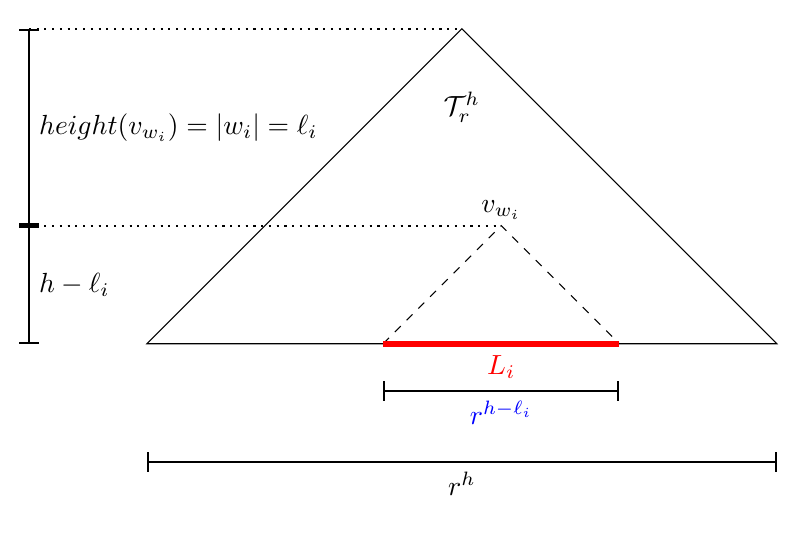
\begin{tikzpicture}
                \node at (0,-1) {$\mathcal{T}_r^h$};
                \node at (.5, -2.3) {$v_{w_i}$};
                \node[color=red] at (.5, -4.3) {$L_i$};

                \draw (0,0)
                    -- (-4,-4)
                    -- (4,-4)
                    -- cycle;

                \draw[dashed] (-1,-4) -- (.5, -2.5) -- (2,-4);

                \draw[line width = 2pt, color=red] (-1,-4) -- (2,-4);

                \draw[dotted, line width = .8pt] (-5.5, -2.5) -- (.5, -2.5);
                \draw[dotted, line width = .8pt] (-5.5, 0) -- (0, 0);
                \draw[|-|, line width = .8pt] (-5.5,-2.5) --
                    node[right] {$height(v_{w_i}) = |w_i| = \ell_i$} (-5.5, 0);
                    \draw[dotted, line width = .8pt] (-5.5, -2.5) -- (.5, -2.5);
                    \draw[|-|, line width = .8pt] (-5.5,-4) -- node[right] {$h-\ell_i$} (-5.5, -2.5);
                \only<2->{
                    \draw[|-|, line width = .8pt] (-1,-4.6) -- node[below,blue] {$r^{h-\ell_i}$} (2,-4.6);
                    \draw[|-|, line width = .8pt] (4,-5.5) -- node[below] {$r^h$} (-4,-5.5);
                }
            \end{tikzpicture}
        \end{center}
\end{frame}

\begin{frame}[t]
    \frametitle{Ungleichung von Kraft: ''$\,\Longleftarrow\,$''}
    \begin{itemize}
        \setlength\itemsep{1em}
        \item $L_i \cap L_j = \varnothing$ für $i \neq j$.
        \item $|L_i| = r^{h-\ell_i}$
    \end{itemize}\strut\\[10pt]

    $$
        r^h \ \geq\ \left| \bigcup_{i \in [1,q]} L_i \right|
    \visible<2->{
        \ =\ \sum_{i=1}^{q} |L_i|
        \ =\ \sum_{i=1}^{q} r^{h-\ell_i}
        \ =\ r^h\sum_{i=1}^{q} \frac{1}{r^{\ell_i}}
    }
    $$
    \visible<3->{
    $$
        \,\Longleftrightarrow\, \sum_{i=1}^{q} \frac{1}{r^{\ell_i}} \leq 1
    $$
    \strut\hfill$\square$
    }
\end{frame}

\begin{frame}[t]
    \frametitle{Ungleichung von Kraft}
    Seien $q,r \in \mathbb{N}, \ell \in \mathbb{N}^q$. Dann existiert ein $r$-ärer sofort dekodierbarer Code $\mathcal{C}$
    mit Wortlängen $\ell$ genau dann, wenn
    $$
        \sum_{k=1}^{q} \frac{1}{r^{l_k}} \leq 1
    $$
    \begin{itemize}
        \setlength\itemsep{1em}
        \item Beweis konstruktiv
        \item Untere Schranke für Wortlänge, Alphabetgröße
        \setlength\itemsep{3em}
        \pause
        \item Bekannt: sofort dekodierbar $\,\Longrightarrow\,$ eindeutig dekodierbar
        \setlength\itemsep{1em}
        \item Schwächere Kriterien?
    \end{itemize}
\end{frame}

\begin{frame}[t]
    \frametitle{Ungleichung von McMillan}
    Seien $q,r \in \mathbb{N}, \ell \in \mathbb{N}^q$. Dann existiert ein $r$-ärer eindeutig dekodierbarer Code $\mathcal{C}$
    mit Wortlängen $\ell$ genau dann, wenn
    \begin{equation}
        K := \sum_{k=1}^{q} \frac{1}{r^{\ell_k}} \leq 1
    \end{equation}\\[20pt]
    \pause

    Richtung ''$(1) \,\Longrightarrow\, \mathcal{C}$ existiert'' durch Kraft.\\
\end{frame}

\begin{frame}[t]
    \frametitle{Ungleichung von McMillan: Beweisidee}
    \begin{itemize}
        \setlength\itemsep{1.3em}
        \item Zu zeigen: $K = \sum_{k=1}^{q} \frac{1}{r^{\ell_k}} \leq 1$
        \item Betrachte $K^n$ abhängig von Wortlängen für beliebiges $n \in \mathbb{N}$.
        \item Finde aus Form von $K^n$ konstante obere Schranke
        \item Dann muss $K \leq 1$, da sonst $K^n$ für geeignetes $n$ größer
            als jede Konstante
    \end{itemize}
\end{frame}

\begin{frame}[t]
    \frametitle{Ungleichung von McMillan: ''$\,\Longleftarrow\,$''}
        Zu zeigen: $K \leq 1$, wobei
        $\displaystyle
            K = \sum_{k=1}^{q} \frac{1}{r^{\ell_k}}
        $.\\
        \pause
        Für $n \in \mathbb{N}$ ist:
        $$
            K^n = \left(\sum_{k=1}^{q} \frac{1}{r^{\ell_k}}\right)^n
            \pause
            = \sum_{i \in [1,q]^n} \prod_{k=1}^{n} \frac{1}{r^{\ell_{i_k}}}
            \pause
            = \sum_{i\in [1,q]^n} r^{-\sum_{k=1}^{n} \ell_{i_k}}
        $$\pause
        Dann für jedes $i \in [1,q]^n:$
        $$
            n\cdot \ell_{min} \leq \sum_{k=1}^{n} \ell_{i_k} \leq n\cdot \ell_{max}
        $$
        \pause
        Wir Wollen schreiben:
        $$
            K^n = \sum_{j=n\cdot \ell_{min}}^{n\cdot \ell_{max}} {\color{red}N_j}\cdot r^{-j}
        $$
\end{frame}

\begin{frame}[t]
    \frametitle{Ungleichung von McMillan: ''$\,\Longleftarrow\,$''}
    Ziel: $K^n$ abschätzen durch Koeffizient ${\color{red}N_j} \in \mathbb{N}_0$, wobei
    $$
        K^n = \sum_{i\in [1,q]^n} r^{-\sum_{k=1}^{n} \ell_{i_k}}
        = \sum_{j=n\cdot\ell_{min}}^{n\cdot\ell_{max}} {\color{red}N_j} \cdot r^{-j}
    $$
    \pause

    \begin{itemize}
        \setlength\itemsep{1em}
        \item $N_j$ Anzahl $i \in [1,q]^n$ mit Wortlängensumme $j$
        \pause
        \item Äquivalent: Anzahl $i \in [1,q]^n$ mit $|w_{i_1}w_{i_2}\dots w_{i_n}| = j$
        \pause
        \item $\mathcal{C}$ eindeutig dekodierbar
            $\,\Longrightarrow\,$ Jede Code-Sequenz aus eindeutiger Auswahl
                $i \in [1,q]^n$
        \pause
    \item $r^j$ Wörter mit Länge $j$, nicht alles Code-Sequenzen von $\mathcal{C}$
    \item Für jedes max. ein $i \in [1,q]^n \,\Longrightarrow\, N_j \leq r^j$
    \end{itemize}

\end{frame}

\begin{frame}[t]
    \frametitle{Ungleichung von McMillan: ''$\,\Longleftarrow\,$''}
        Mit {\only<2>{\color{red}}$N_j \leq r^j$} folgt:
        $$
            K^n =
            \sum_{i\in [1,q]^n} r^{-\sum_{k=1}^{n} \ell_{i_k}}
            = \sum_{j = nm}^{nM} N_jr^{-j}
            = \sum_{j = nm}^{nM} \frac{N_j}{r^j}
        $$
        \pause
        $$
            \quad{\color{red}\leq}\quad \sum_{j = nm}^{nM} 1
            = (M-m)n + 1
        $$
        \pause
        $$
            \,\Longrightarrow\, \frac{K^n}{n} \leq (M-m) + 1
        $$
\end{frame}

\begin{frame}[t]
    \frametitle{Ungleichung von McMillan: ''$\,\Longleftarrow\,$''}
        $$
            \frac{K^n}{n} \leq (M-m) + 1
        $$
        \begin{itemize}
            \setlength\itemsep{1em}
            \item Code $\mathcal{C}$ gegeben; $q = |\mathcal{C}|$, Alphabetgröße $r$, Wortlängen $\ell$ fix.
            \item Damit auch $m,M,K$ fix.
            \pause
            \item $n \in \mathbb{N}$ beliebig; Ungleichung muss für alle $n \in \mathbb{N}$ gelten.
            \pause
            \item Nach Analysis bekannt: nur möglich für $K \leq 1$.
        \end{itemize}
        \strut\\[10pt]
        $$
            \,\Longrightarrow\, \sum_{i=1}^{q} \frac{1}{r^{\ell_i}} = K \leq 1
        $$
        \strut\hfill$\square$
\end{frame}

\end{document}
